\documentclass[12pt,fleqn]{article}\usepackage{../../common}
\begin{document}
Zaman Serisi Veri Analizi

Daha fazla ilerlemeden bu yazıda bazı veri işlem numaraları göreceğiz.

Trend Çıkartmak (Detrending)

Bazen bir zaman serisi verisinde genel gidişata değil diğer değişikliklere
odaklanmak istiyoruz. O zaman genel gidişat, yani trendi veriden
çıkartabiliriz. Örnek olarak Apple şirketinin borsa fiyatlarını kullanalım.

\begin{minted}[fontsize=\footnotesize]{python}
import pandas as pd
df = pd.read_csv('AAPL.csv').reset_index()
\end{minted}

Veri üzerinde lineer regresyon yaparız. LR tanım itibariyle veriye bir düz çizgi
uydurduğu (fit) için, bu düz çizgiyi alıp veriden çıkartarak trend çıkartma
işlemi olarak kullanabiliriz. Ama LR katsayılarına dalmadan önce şunu düşünelim,
LR'de yan ürün olarak hesaplanan artıklar (residuals) aslında lineer çizgi ile
gerçek verinin farkı değil midir? O zaman bu artıklar zaten verinin trend
çıkartılmış halidir!

\begin{minted}[fontsize=\footnotesize]{python}
import statsmodels.formula.api as smf
results = smf.ols('AAPL ~ index', data=df).fit()
df['AAPL Trendsiz'] = results.resid
df[['AAPL','AAPL Trendsiz']].plot()
plt.savefig('tser_008_data_02.png')
\end{minted}

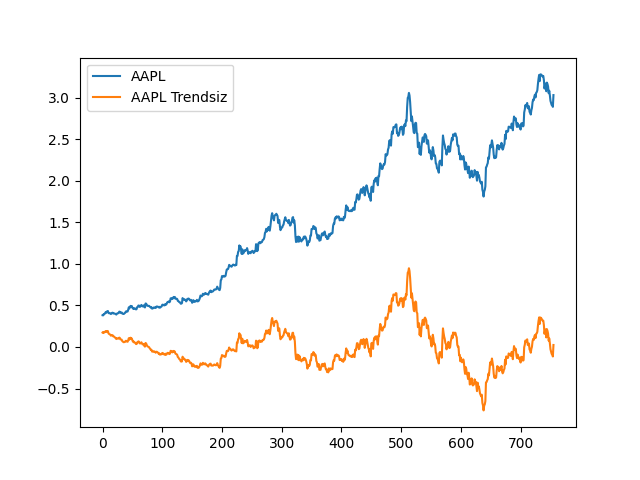
\includegraphics[height=6cm]{tser_008_data_02.png}

Trend çıkarılmış grafik için \verb!resid! verisi kullanıldı çünkü bu değişken
içinde model ile gerçek değerler arasındaki fark, 'artıklar' gösteriliyor, ki
bu dolaylı olarak veriden trend çıkartılmış hal demektir.

Fark Hesabi ile Trend Cikartmak

Fakat belki de en basit trend cikartma yontemi basit fark hesabi.

\begin{minted}[fontsize=\footnotesize]{python}
import pandas as pd
df = pd.read_csv('AAPL.csv',index_col=0).reset_index()
df.AAPL.diff().dropna().plot()
plt.savefig('tser_008_data_03.png')
\end{minted}

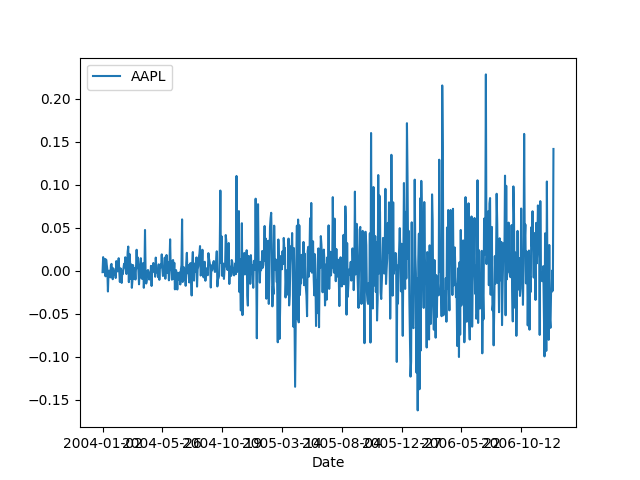
\includegraphics[height=6cm]{tser_008_data_03.png}



Durağanlığı Çıkartmak

Yapay Öğrenim (machine learning) ya da diğer istatistiki tahminsel yaklaşımlar
çoğunlukla işledikleri verinin durağan olmasının beklerler [1]. Durağanlık
zaman serisindeki her veri noktasının diğerleri ile aynı dağılıma sahip olması
demektir. Bunun tersini farzeden algoritmalar için bu rahatsızlık yaratır. 

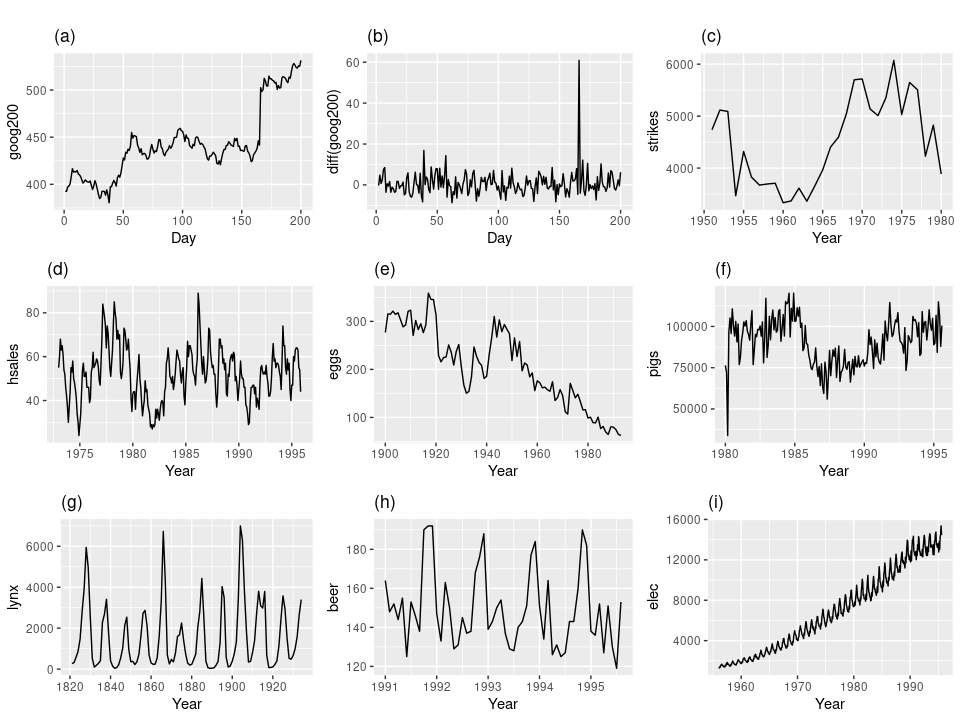
\includegraphics[width=25em]{tser_008_data_01.png}











[devam edecek]

Kaynaklar

[1] {\em How to Remove Non-Stationarity From Time Series},
    \url{https://www.kaggle.com/code/bextuychiev/how-to-remove-non-stationarity-from-time-series?scriptVersionId=73876070}

\end{document}
